\subsection{www.cam.ac.uk}

En esta ocasión se envió un paquete ICMP con destino hacia la URL \textit{www.cam.ac.uk}, donde está hosteado el sitio de la Universidad de Cambridge en el Reino Unido. Con el fin de obtener los nodos distinguidos, posteriormente se calculo el Z-Score en base a los resultados obtenidos con la herramienta implementada para este trabajo práctico.
En esta primera figura se puede ver el viaje que realizó el paquete hasta arribar a su destino, deduciendo la ubicación geográfica de los hops intermedios a partir de sus direcciones IP.

\begin{landscape}
\begin{figure}[H]
  \centering	
	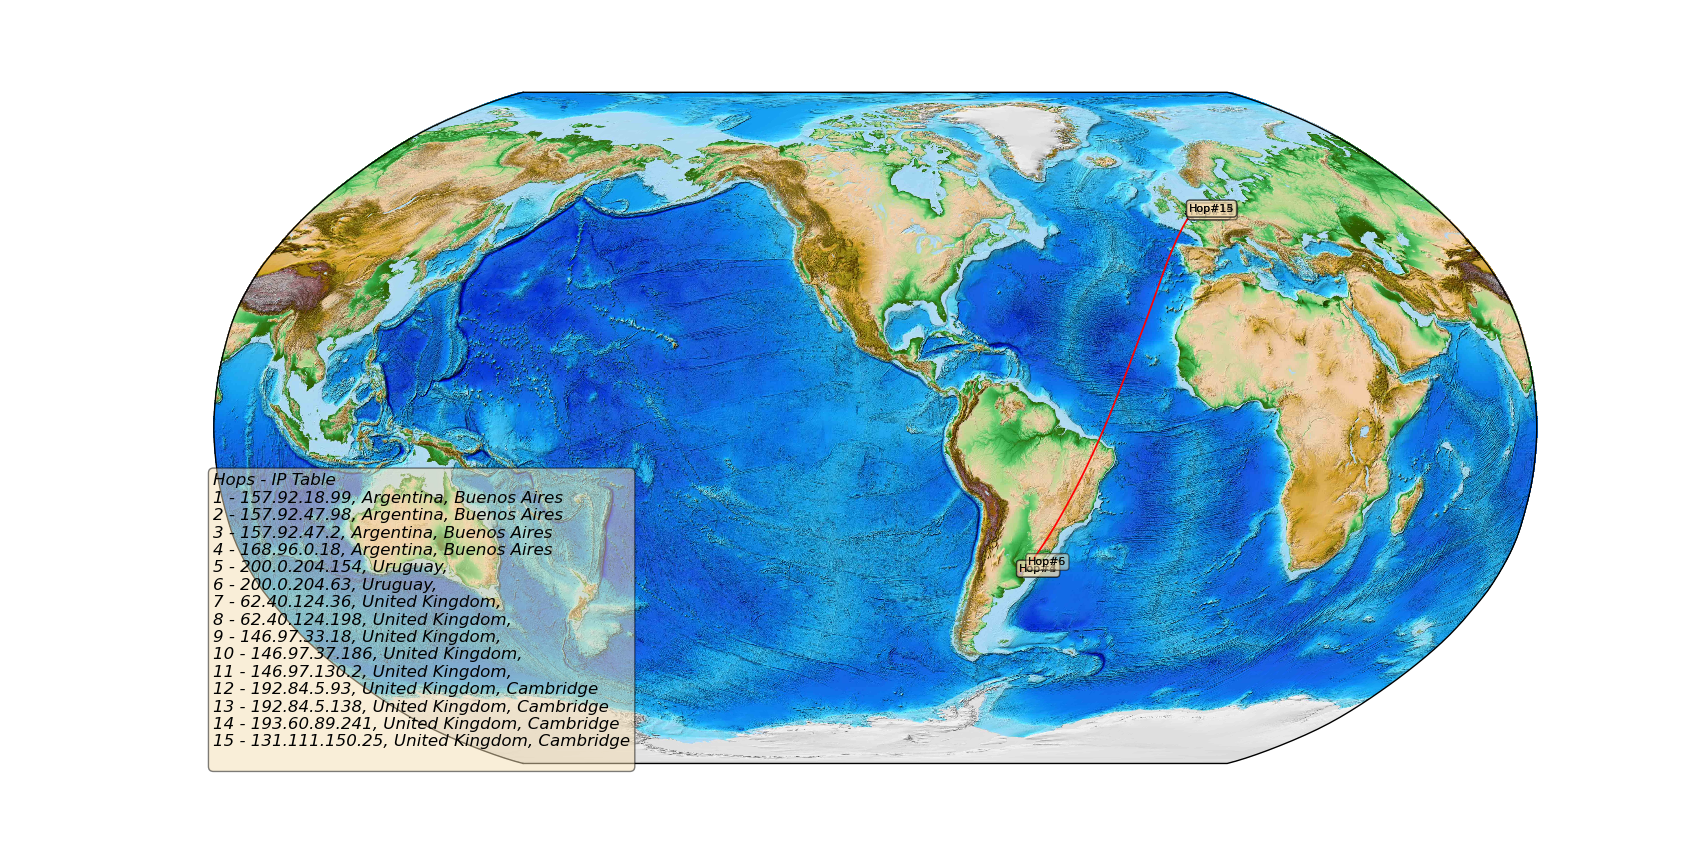
\includegraphics[scale=0.5]{../cambridge-experiment/figure_1.png}
  \caption{Planisferio donde se puede ver el trayecto realizado por el paquete en rojo.}
	\label{fig:histo-src-sitiotrabajo}
\end{figure}
\end{landscape}

En los siguientes gráficos se hallan los valores asociados a los \textit{Round Trip Time} que se estimaron entre cada uno de los nodos. En el primero de ellos se muestra el \textit{RTT} entre dos nodos consecutivos, mientras que en el segundo se puede apreciar el acumulado de estos a medida que el paquete se acerca al destino.

\begin{figure}[H]
  \centering	
	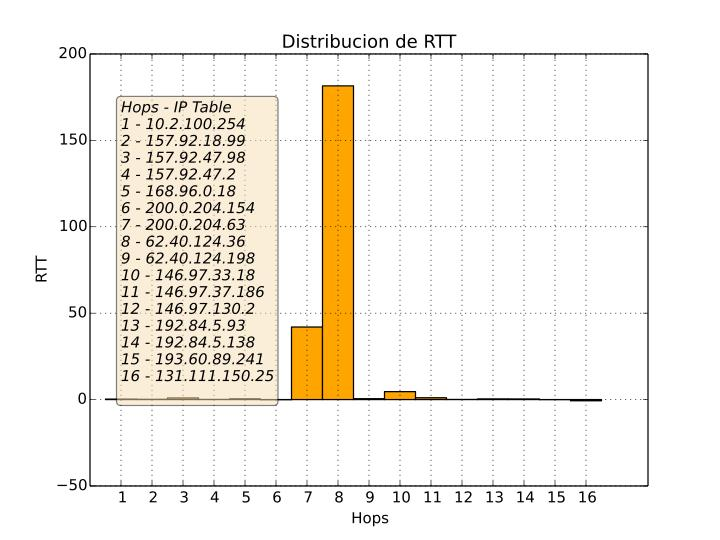
\includegraphics[scale=0.4]{../cambridge-experiment/bar_rtt.jpeg}
  \caption{RTT entre dos hop consecutivos medido en milisegundos.}
	\label{fig:histo-src-sitiotrabajo}
\end{figure}

\begin{figure}[H]
  \centering	
	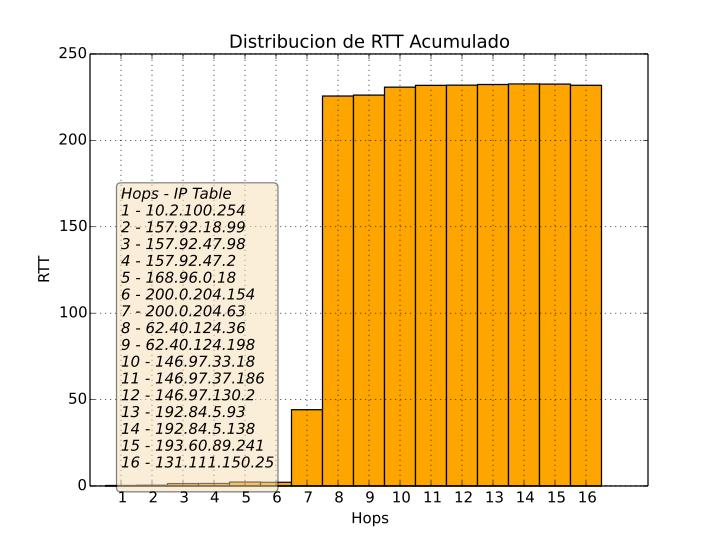
\includegraphics[scale=0.4]{../cambridge-experiment/bar_rtt_acum.jpeg}
  \caption{RTT acumulado del paquete a medida que avanza en su camino hacia la Universidad de Cambridge.}
	\label{fig:histo-src-sitiotrabajo}
\end{figure}

Finalmente, los resultados obtenidos por el Z-Score permiten distinguir a los saltos de mayor importancia en el trayecto, como era de esperarse estos están relacionados con el del salto transoceánico que se realiza entre Uruguay y el Reino Unido.

\begin{figure}[H]
  \centering	
	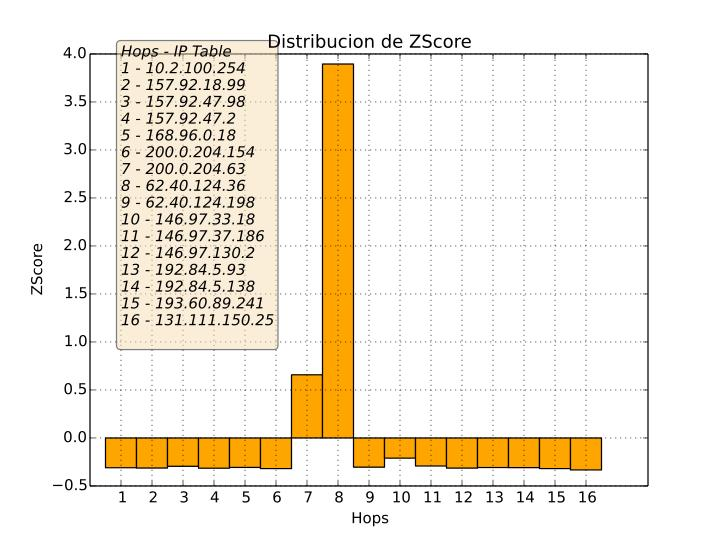
\includegraphics[scale=0.4]{../cambridge-experiment/bar_z_score.jpeg}
  \caption{Z-Score para cada uno de los saltos.}
	\label{fig:histo-src-sitiotrabajo}
\end{figure}

\subsubsection{Tabla de Hops de la traza}
\begin{center}
  \resizebox{\textwidth}{!}{\begin{tabular}{| c | c | c | c | c | c |}
		\hline
		Hop Score & Hop Ip & RTT Acum & RTT Incr & Hop Location & Hop Name\\
		\hline
		-0.31 & 10.2.100.254 & 0.29 & 0.29 & -,  & -\\
		\hline
		-0.313 & 157.92.18.99 & 0.44 & 0.15 & Argentina, Buenos Aires & ccc-pab2.fcen.uba.ar.\\
		\hline
		-0.295 & 157.92.47.98 & 1.38 & 0.94 & Argentina, Buenos Aires & -\\
		\hline
		-0.315 & 157.92.47.2 & 1.45 & 0.07 & Argentina, Buenos Aires & -\\
		\hline
		-0.307 & * & * & 0.41 & - & -\\
		\hline
		-0.307 & 168.96.0.18 & 2.27 & 0.41 & Argentina, Buenos Aires & rnoc8a.innova-red.net.\\
		\hline
		-0.319 & 200.0.204.154 & 2.14 & -0.13 & Uruguay,  & ar-inova.redclara.net.\\
		\hline
		0.658 & 200.0.204.63 & 44.13 & 41.99 & Uruguay,  & br-ar.redclara.net.\\
		\hline
		3.895 & 62.40.124.36 & 225.67 & 181.54 & United Kingdom,  & redclara.lon.uk.geant.net.\\
		\hline
		-0.304 & 62.40.124.198 & 226.19 & 0.52 & United Kingdom,  & janet-gw.mx1.lon.uk.geant.net.\\
		\hline
		-0.21 & 146.97.33.18 & 230.79 & 4.6 & United Kingdom,  & ae28.lowdss-sbr1.ja.net.\\
		\hline
		-0.292 & 146.97.37.186 & 231.84 & 1.05 & United Kingdom,  & ae0.camb-rbr2.ja.net.\\
		\hline
		-0.314 & 146.97.130.2 & 231.94 & 0.1 & United Kingdom,  & University-of-Cambridge.Camb-rbr1.eastern.ja.net.\\
		\hline
		-0.308 & 192.84.5.93 & 232.32 & 0.38 & United Kingdom, Cambridge & route-enet.route-mill.net.cam.ac.uk.\\
		\hline
		-0.309 & 192.84.5.138 & 232.66 & 0.34 & United Kingdom, Cambridge & route-mill.route-nwest.net.cam.ac.uk.\\
		\hline
		-0.319 & 193.60.89.241 & 232.57 & -0.09 & United Kingdom, Cambridge & mint.admin.cam.ac.uk.\\
		\hline
		-0.333 & 131.111.150.25 & 231.86 & -0.71 & United Kingdom, Cambridge & primary.admin.cam.ac.uk.\\
		\hline
	\end{tabular}}
\end{center}

\subsubsection{Tabla de Hops Distinguidos}
\begin{center}
  \resizebox{\textwidth}{!}{\begin{tabular}{| c | c | c | c | c | c |}
		\hline
		Hop Score & Hop Ip & RTT Acum & RTT Incr & Hop Location & Hop Name\\
		\hline
		0.658 & 200.0.204.63 & 44.13 & 41.99 & Uruguay,  & br-ar.redclara.net.\\
		\hline
		3.895 & 62.40.124.36 & 225.67 & 181.54 & United Kingdom,  & redclara.lon.uk.geant.net.\\
		\hline
	\end{tabular}}
\end{center}

\subsubsection{Estadistica sobre las mediciones de RTT incremental}
\begin{itemize}
	\item $\overline{RTT_i}: 13.639$
	\item $STDEV(RTT_i): 43.102$
\end{itemize}

\subsubsection{Conclusion y aclaraciones}
Para este experimento coincidieron perfectamente los resultados obtenidos con las herramientas de geolocalización de direcciones IP y los datos arrojados por los estimadores estadistícos. Se puede ver en el planisferio el salto dentro de Uruguay de mediana distancia(Hops 6 y 7 en grafico de RTT incremental y Zscore), asi también se observa la variacion de RTT entre los hops de Uruguay y Reino Unido de larga distancia en el planisferio (Hops 7 y 8 en el grafico de RTT incremental y Zscore). Estos son los 2 saltos de mayor distincion en la traza, y quedaron al descubierto con ambas herramientas utilizadas.
